\chapter{连续函数}

本节课主要介绍函数的连续性.连续函数有很多好的性质,在今后微分和积分的学习中有重要作用.我们已经学习过函数极限,函数连续性也是在函数极限的基础上定义的.

本节课主要内容包括:
\begin{enumerate}
	\item 函数连续性的概念;
	\item 连续函数的运算;
	\item 闭区间连续函数的性质;
	\item 函数的一致连续性.
\end{enumerate}

\section{函数的连续性概念与间断点的分类}
\subsection{函数的连续性概念}
我们见过的很多初等函数,例如$y=x^2,y=\sin x,y=\sqrt{x},y=\left|x\right|$等等,在定义域内都是连续函数;同时,我们也遇到过一些不连续的函数,例如:

Dirichlet函数:
\[
	f(x) =
	\begin{cases}
		0 & x \text{为无理数} , \\
		1 & x \text{为有理数} .
	\end{cases}
\]

取整函数$f(x)=[x]$,如图\ref{roundfun}.
\begin{figure}[H]
	\centering
	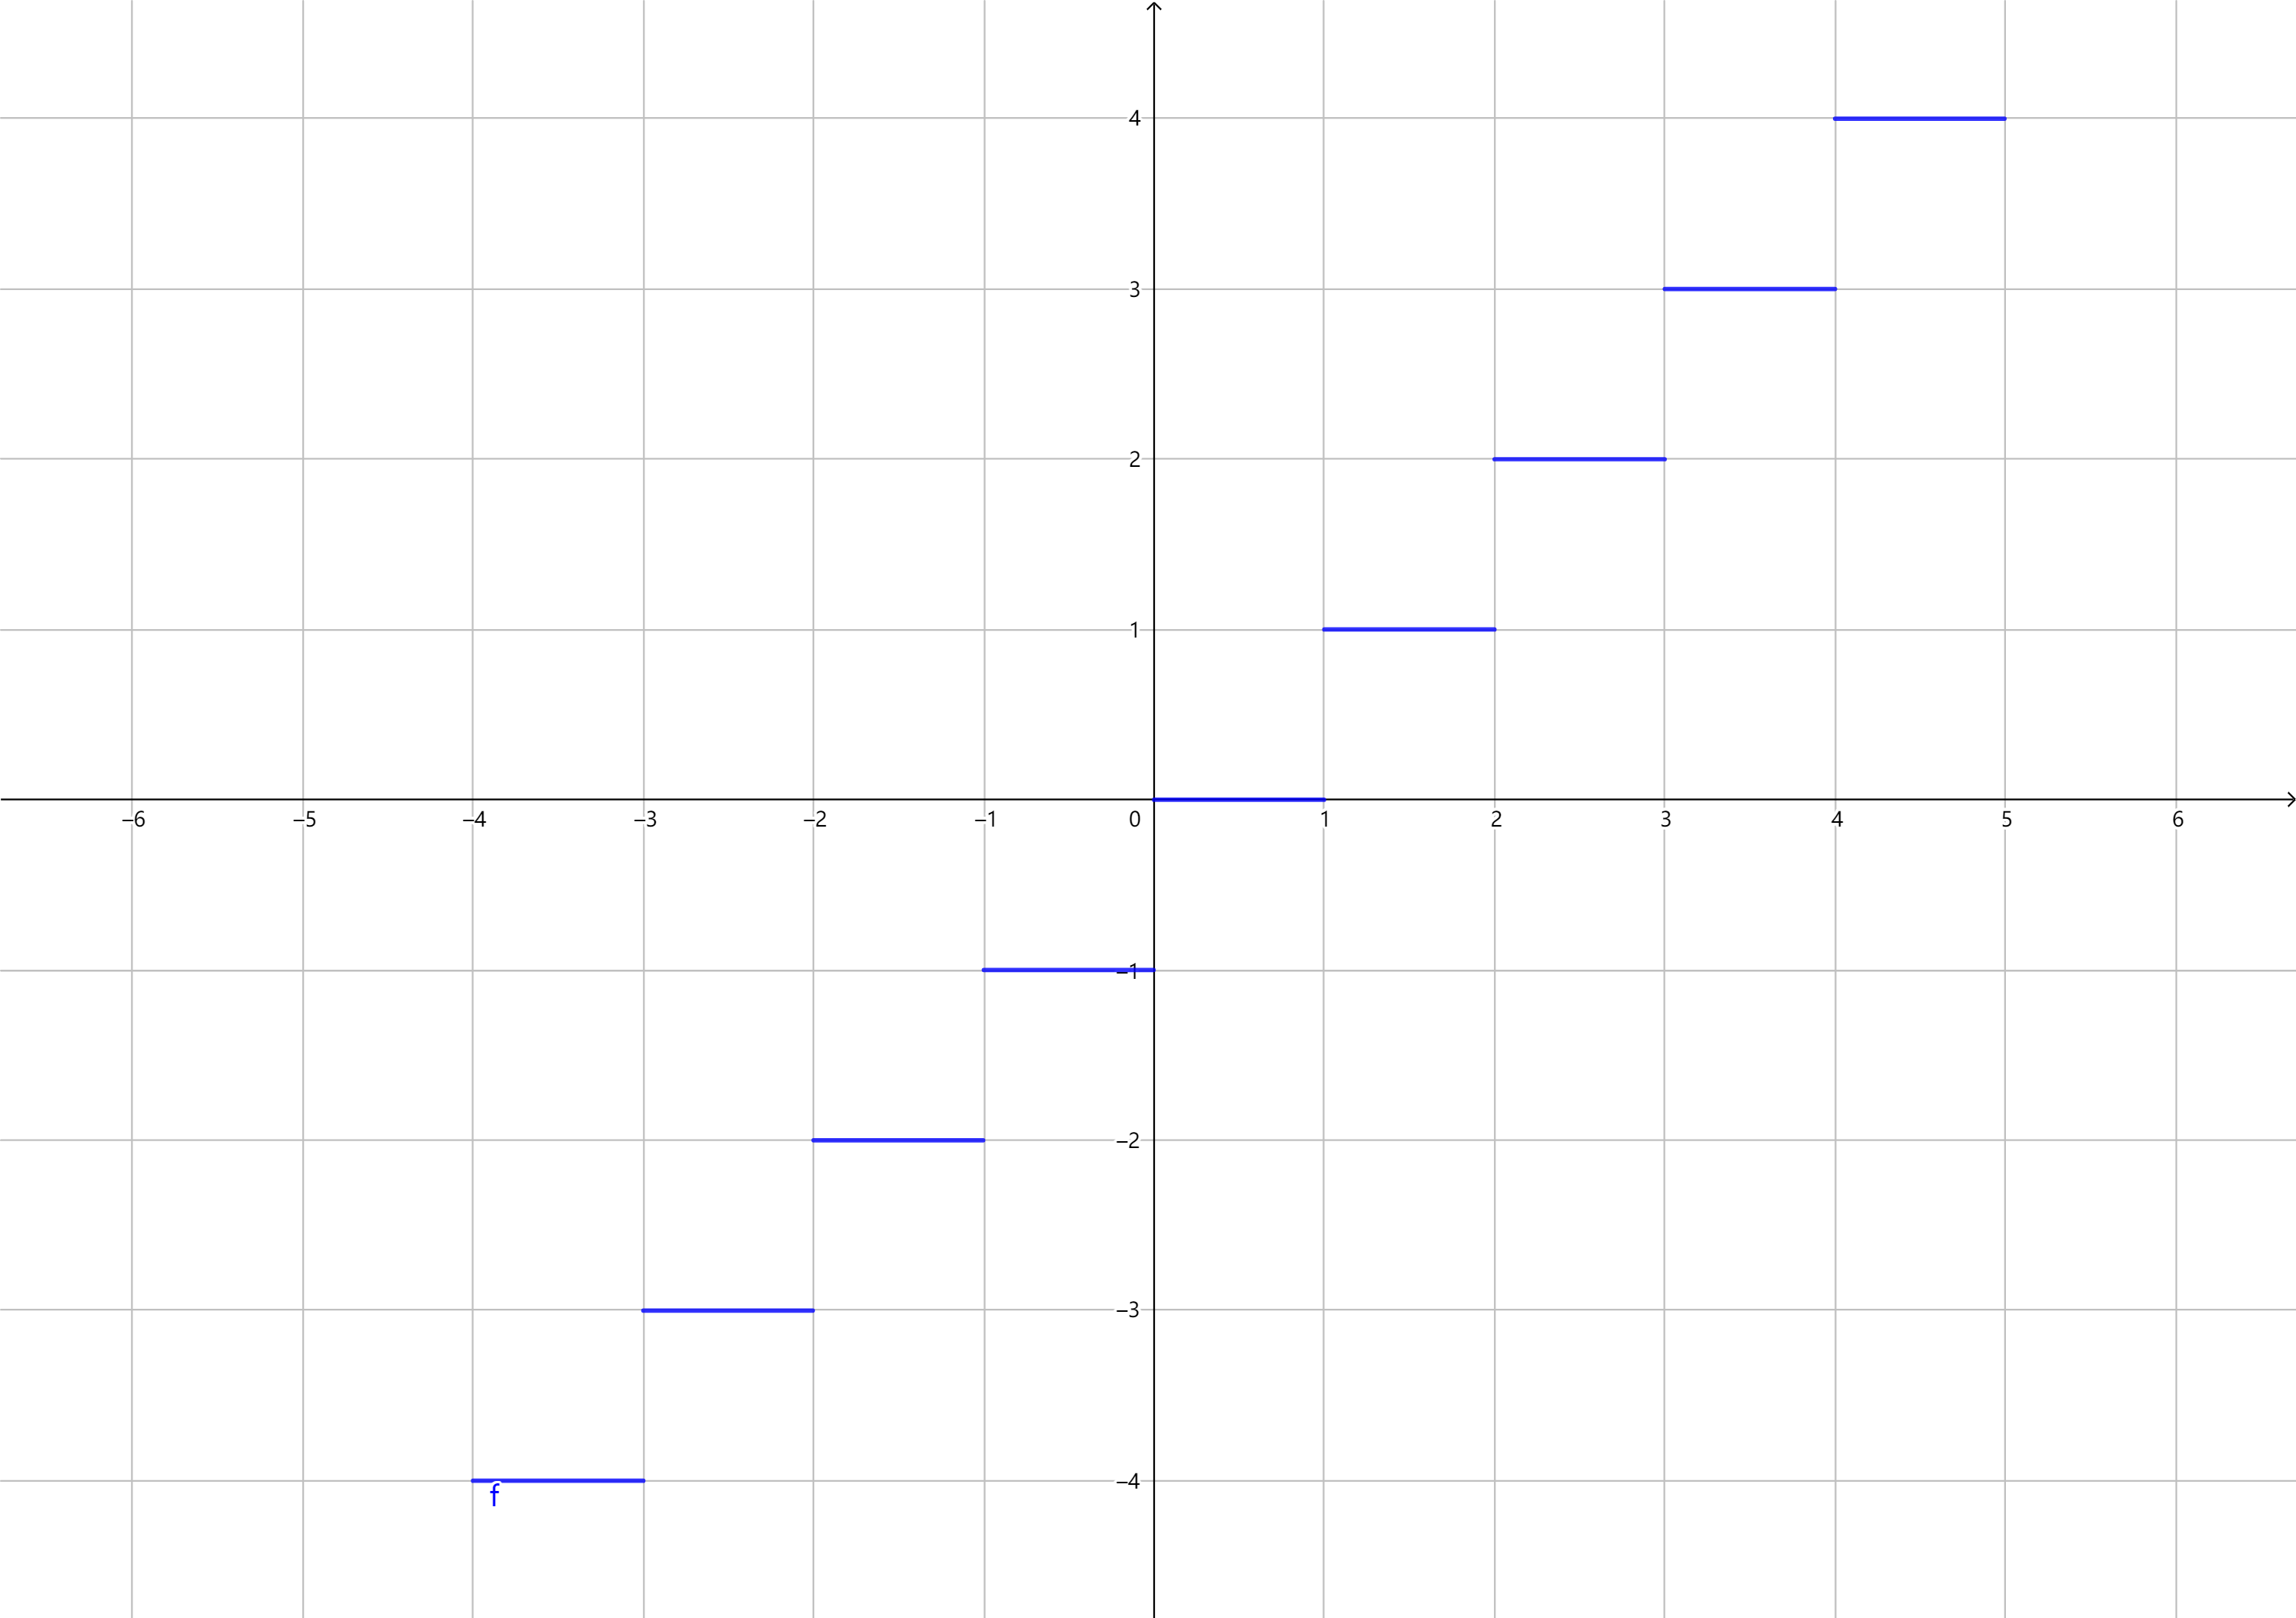
\includegraphics[width=0.6\textwidth]{figures/roundfun}
	\caption{$f(x)=[x]$图像}\label{roundfun}
\end{figure}

由这几个例子,我们可以明显看出连续函数和不连续函数的区别.连续函数的自变量改变量$\Delta x\to 0$时,因变量的改变量$\Delta y\to 0$.而不连续函数的自变量改变量$\Delta x\to 0$时,函数值可能发生跳跃,函数值的极限不趋于0.基于此,我们可以这样来定义连续函数:

\begin{definition}[\textbf{连续函数}]
	设函数f定义在$\left[a,b\right]$上,对于任意一点$x_{0}\in \left(a,b\right)$,若对于任意给定的$\epsilon>0$,存在$\delta>0$,使得对于任意满足$\left|x-x_0\right|<\delta$的x,有
	\[
		\left|f(x)-f(x_0)\right|<\epsilon
	\]
	那么就称函数f在$x_0$处连续,如果f在$\left[a,b\right]$中每一点都连续,那么就称函数f在区间$\left[a,b\right]$上连续.
\end{definition}

我们记在区间$I$上连续函数的全体构成的集合为$C(I)$.

类似左极限和右极限,我们也可以来定义左连续和右连续.
\begin{enumerate}
	\item 左连续:$\lim\limits_{x\to x_{0}^{-}}f(x)=f(x_0)$;
	\item 右连续:$\lim\limits_{x\to x_{0}^{+}}f(x)=f(x_0)$;
\end{enumerate}

\begin{theorem}
	函数在某一点处连续当且仅当函数在这一点处既左连续又右连续.
\end{theorem}

\subsection{间断点的分类}
我们已经讨论了连续函数,下面还需要讨论一个函数不连续的情况.

如果函数$f$在$x_0$处不连续,那么这个函数就不是连续函数,所以我们要研究不连续点的情况.

\begin{definition}[\textbf{函数的间断点}]
	设函数$f$在$x_0$的某一单侧邻域内有定义,若$f$在$x_0$不连续,那么称$x_0$是$f$的一个间断点.
\end{definition}
根据函数间断点的特征,有以下几个分类:

\begin{enumerate}
	\item \textbf{可去间断点}:$\lim\limits_{x\to x_0^{-}}f(x)=\lim\limits_{x\to x_0^{+}}f(x)\ne f(x_0)$
	      \begin{example}
		      \[
			      f(x) =
			      \begin{cases}
				      \frac{x^{2}-1}{x-1} & x \ne 1 , \\
				      1                   & x =1 .
			      \end{cases}
		      \]
		      由于$\lim\limits_{x\to 1}f(x)=2\ne f(x)$,所以$x=1$是$f$的一个可去间断点.
	      \end{example}

	\item \textbf{跳跃间断点}:$\lim\limits_{x\to x_0^{-}}f(x)\ne \lim\limits_{x\to x_0^{+}}f(x)$.
	      \begin{example}
		      \[
			      f(x) =
			      \begin{cases}
				      x^2+1 & x <0,  \\
				      0     & x =0 , \\
				      x-1   & x>0.
			      \end{cases}
		      \]
		      由于$\lim\limits_{x\to 0^-}f(x)=1\ne\lim\limits_{x\to 0^+}f(x)=-1,$所以$x=0$ 是$f$的一个跳跃间断点.
	      \end{example}

	\item \textbf{无穷间断点}:$\lim\limits_{x\to x_0^{-}}$与$\lim\limits_{x\to x_0^{+}}$至少有一个是无穷.
	      \begin{example}
		      \[
			      f(x)=\frac{1}{x^2}
		      \]
		      由于当$x\to 0$时,$f(x)\to +\infty$,故$x=0$是$f$的无穷间断点.
	      \end{example}

	\item \textbf{振荡间断点}:$\lim f(x)$振荡不存在.
	      \begin{example}
		      \[
			      f(x)=\sin\frac{1}{x}
		      \]
		      由于当$x\to 0$时,$f(x)$极限不存在,故$x=0$是$f$的一个振荡间断点.
	      \end{example}
\end{enumerate}

我们也将以上四类情况分为两大类:
\begin{enumerate}
	\item \textbf{第一类间断点}:函数左右极限都存在的间断点.
	      包括:可去间断点和跳跃间断点.
	\item \textbf{第二类间断点}:函数左右极限至少有一个不存在.
	      包括:无穷间断点和振荡间断点.
\end{enumerate}

\section{连续函数的运算性质与初等函数的连续性}
\subsection{连续函数的运算性质}
由于函数的连续性是基于函数极限定义的,因此函数极限的某些性质对于连续函数依然适应.

\begin{theorem}[\textbf{四则运算}]
	若$f,g$在$x_0$处连续,则$f\pm g,fg,\frac{f}{g}(g(x_0)\ne 0)$在$x_0$处都连续
\end{theorem}

\begin{theorem}[\textbf{局部有界性}]
	若$f$在$x_0$处连续,则$f$在$x_0$处是局部有界的.
\end{theorem}

\begin{theorem}[\textbf{复合函数的连续性}]
	设$y=f(g(x))$是由$y=f(u)$与$u=g(x)$复合而成的,$x_0\in D(f\circ g).$若$g$在$x_0$处连续,$f$在对应的$g(x_0)$处连续,且$u_0=g(x_0)$,则复合函数$y=f(g(x))$也在$x_0$处连续.
\end{theorem}

\begin{theorem}[\textbf{反函数的连续性}]
	设$f:I\to \mathbb{R}$是严格单调的连续函数,则其反函数$f^{-1}$存在,并且在$f(I)$上也是严格单调的连续函数.
\end{theorem}

根据反函数连续性定理,容易证明反三角函数,对数函数,幂函数在各自的定义区间上连续.

\subsection{初等函数的连续性}

我们容易证明:\textbf{所有初等函数在它们的定义域内的任何区间上都是连续的}

同时,有以下定理:
\begin{theorem}
	由初等函数的有限次四则运算构成的函数为初等函数且连续.
\end{theorem}
至此,可以得到我们见过的很多函数在其定义域内是连续的.
基于此,我们给出以下例题:
\begin{example}
	讨论
	\begin{equation*}
		f(x) =
		\begin{cases}
			e^{\frac{1}{x-1}} & x >0,      \\
			\ln{(1+x)}-1      & 1<x\le 0 .
		\end{cases}
	\end{equation*}
	的连续性。
\end{example}
\begin{solution}
	在$x=0$处,$\lim\limits_{x\to 0^-}f(x)=0\ne \lim\limits_{x\to 0^+}f(x)=\frac{1}{e}$,故$x=0$是第一类间断点;

	在$x=1$处,$\lim\limits_{x\to 1^+}f(x)=+\infty,$故$x=1$是第二类间断点;

	在其他定义域内,显然$f(x)$连续.
\end{solution}

根据以上性质和复合函数连续性定理,我们可以得到以下等式:
\[
	\lim_{x\to x_0}f(g(x))=f(g(x_0))=f(\lim_{x\to x_0}g(x)).
\]

这说明,在求连续函数极限的过程中,\textbf{极限符号可以与函数符号交换次序}.

基于此,我们容易验证以下等式:
\begin{example}
	\[
		\lim_{x\to 0}\frac{\ln{(1+x)}}{x}=1;
	\]\[
		\lim_{x\to 0}\frac{e^{x}-1}{x}=1;
	\]\[
		\lim_{x\to 0}\frac{(1+x)^{\alpha}-1}{x}=\alpha.
	\]
\end{example}

下面我们再给出一些特殊函数的连续性,同学们可以思考它们为何连续或不连续.
\begin{example}
	Dirichlet函数在$\mathbb{R}$上每个点处都不连续.
\end{example}
\begin{example}
	Riemann函数只在无理点连续.
\end{example}
\begin{example}
	记$D(x)$为Dirichlet函数,则$xD(x)$只在$x=0$处连续.
\end{example}

\subsection{幂指函数的连续性与极限}
设函数$f,g,f>0$.则
\[
	\lim f(x)^{g(x)}=e^{\lim g(x)\ln{f(x)}}
\]

这就将幂指函数的极限问题转化为$g(x)\ln f(x)$的极限问题.

例如下面这道例题:
\begin{example}
	求$\lim\limits_{x\to +\infty}(1+\frac{1}{x^2})^{\sqrt{x}}$.
\end{example}

\begin{solution}
	\[
		\lim_{x\to +\infty}(1+\frac{1}{x^2})^{\sqrt{x}}=e^{\lim\limits_{x\to +\infty}\sqrt{x}\ln{(1+\frac{1}{x^2})}}=e^{\lim\limits_{x\to +\infty}\frac{\sqrt{x}}{x^2}}=e^0=1.
	\]
\end{solution}

\section{闭区间上连续函数的性质}
闭区间上的连续函数有很多好的性质,这些性质有很重要的作用.
\begin{theorem}[\textbf{有界性}]
	设$f\in C\left[a,b\right]$,则$f$在$\left[a,b\right]$上有界.
\end{theorem}
这是一个很显然的性质,类似地,我们可以得到以下定理:
\begin{theorem}[\textbf{最大值最小值定理}]
	设$f\in C\left[a,b\right]$,则$f$在$\left[a,b\right]$上一定可以取到它的最大值与最小值.
\end{theorem}
由最大值最小值定理,我们也很容易推出闭区间连续函数的有界性定理.

下面一个定理是零点存在定理,高中已经接触过这个定理,这里我们将更严格地给出这个定理.
\begin{theorem}[\textbf{零点存在定理}]
	设$f\in C\left[a,b\right]$,若$f(a)f(b)<0$,则至少存在一点$\xi \in \left(a,b\right)$,使$f(\xi)=0$.
\end{theorem}
零点存在性定理可以用闭区间套定理来证明,这是闭区间套定理的一个典型应用,它的证明过程是利用\textbf{二分法},一种非常常见的求方程近似解的方法,同学们可以注意一下这个证明过程.
\begin{example}
	设$f\in C\left[0,1\right],$且$0<f(x)<1$.证明:存在$\xi\in\left(0,1\right)$,使得$f(\xi)=\xi$.
\end{example}
\begin{proof}
	设$F(x)=f(x)-x,$由于$F(0)=f(0)-0>0,F(1)=f(1)-1<0$,

	所以,由零点存在性定理可知:

	存在$\xi\in\left(0,1\right)$,使得$F(\xi)=0$,

	即,存在$\xi\in\left(0,1\right)$,使得$f(\xi)=\xi$.

\end{proof}

我们得到零点存在性定理之后,很容易可以证明介值定理:
\begin{theorem}[\textbf{介值定理}]
	设$f\in C\left[a,b\right],$如果存在$\eta $使$f(a)<\eta <f(b)$,则存在$\xi\in\left(a,b\right)$,使$f(\xi)=\eta$.
\end{theorem}
介值定理也可以理解为:闭区间上连续函数一定可以取到介于最大值和最小值之间的值.

\begin{theorem}
	闭区间连续函数把区间映成区间或单点集.
\end{theorem}
这个定理可以理解为:闭区间上的连续函数的函数值一定连续不断地充满它的值域.

\section{函数的一致连续性}
函数的一致连续性在高数中不做重点要求.但是,函数的一致连续性理论对于以后严格地讨论级数等相关理论有重要作用.下面将简单介绍函数的一致连续性.

我们已经给出过连续函数的定义.回顾函数连续的定义,我们会发现,定义中$\delta$的选取同时与$\epsilon$和$x_0$有关.我们思考,是否存在这样的连续函数,使得对于任意给定的正数$\epsilon$,可以选取同一个$\delta$满足条件.

我们想要的这类连续函数就被称为一致连续函数,下面给出一致连续函数的定义:
\begin{definition}[\textbf{一致连续函数}]
	设$f$在区间$I$上有定义,如果对于任意正数$\epsilon$,存在正数$\delta$,使得对于任意的$x,y\in I$,只要$\left|x-y\right|<\delta$,就有$\left|f(x)-f(y)\right|<\epsilon$.则称$f$在$I$上一致连续.
\end{definition}

我们可以这样区分连续和一致连续:
\begin{itemize}
	\item 连续研究的是函数局部的性质,也就是在某一点附近的性质;
	\item 一致连续研究的是函数整体的性质,在整个定义域区间的性质.
\end{itemize}

最后,我们给出一致连续函数的一个重要定理:
\begin{theorem}[\textbf{Cantor定理}]
	闭区间上的连续函数是一致连续的.
\end{theorem}
这个定理可以让我们更容易判断一些常见函数的一致连续性,同时也是闭区间连续函数的一条重要性质.